% !TEX root = ../main.tex
	 
\chapter{Wireframes of Survey Application}\label{ap:wireframes}

  \begin{figure}[H]
    \centering
    \subfigure[Introduction screen]{
      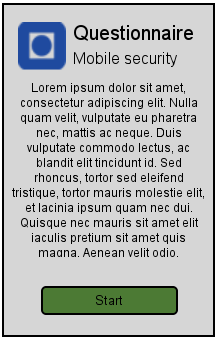
\includegraphics[scale=0.48]{pics/wireframes/plain1-1.png}
      \label{fig:wireframe1}
    }
    \subfigure[Introduction to Android Lock Pattern]{
      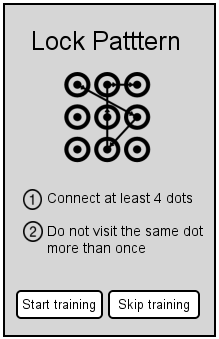
\includegraphics[scale=0.48]{pics/wireframes/plain1-2.png}
      \label{fig:wireframe2}
    }
    \subfigure[Training mode]{ 
      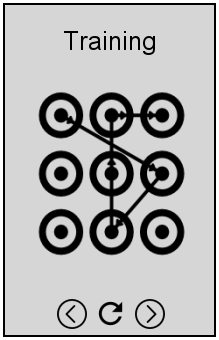
\includegraphics[scale=0.48]{pics/wireframes/plain1-3.png}
      \label{fig:wireframe3}
    }
    \subfigure[Introduction to pattern creation]{
      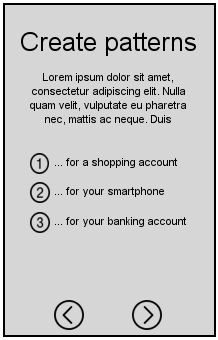
\includegraphics[scale=0.48]{pics/wireframes/plain1-4.png}
      \label{fig:wireframe4}
    }
    \subfigure[Creation of pattern 1]{
      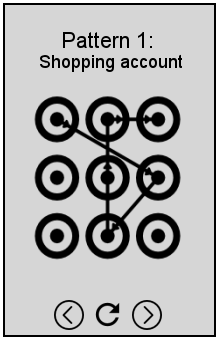
\includegraphics[scale=0.48]{pics/wireframes/plain1-5.png}
      \label{fig:wireframe5}
    }
    \subfigure[Creation of pattern 2]{
      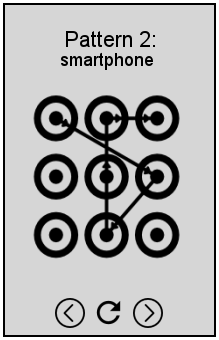
\includegraphics[scale=0.48]{pics/wireframes/plain1-6.png}
      \label{fig:wireframe6}
    }
  \end{figure}

  \begin{figure}[H]
    \centering
    \subfigure[Creation of pattern 3]{
      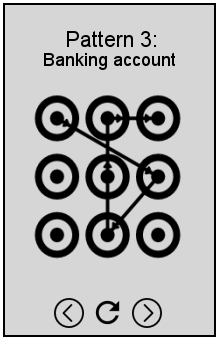
\includegraphics[scale=0.48]{pics/wireframes/plain1-7.png}
      \label{fig:wireframe7}
    }
    \subfigure[Q1: Hand size]{
      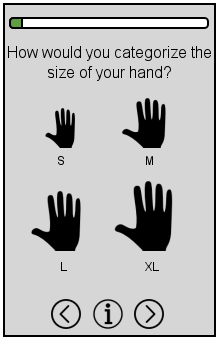
\includegraphics[scale=0.48]{pics/wireframes/plain2-1.png}
      \label{fig:wireframe8}
    }
    \subfigure[Q2: Screen size]{
      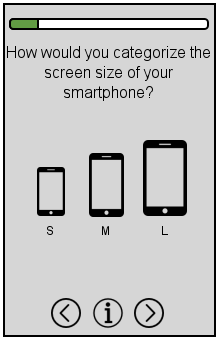
\includegraphics[scale=0.48]{pics/wireframes/plain2-2.png}
      \label{fig:wireframe9}
    }
    \subfigure[Q3: Handedness]{
      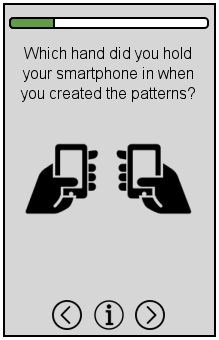
\includegraphics[scale=0.48]{pics/wireframes/plain2-3.png}
      \label{fig:wireframe10}
    }
    \subfigure[Q4: Finger used in pattern creation]{
      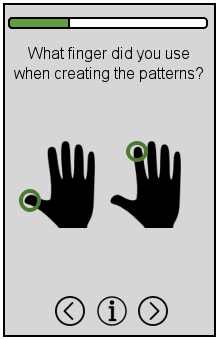
\includegraphics[scale=0.48]{pics/wireframes/plain2-4.png}
      \label{fig:wireframe11}
    }
    \subfigure[Q5: Reading/Writing orientation]{
      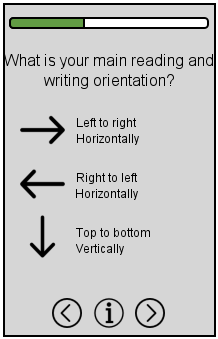
\includegraphics[scale=0.48]{pics/wireframes/plain2-5.png}
      \label{fig:wireframe12}
    }
    \subfigure[Q6: Gender]{
      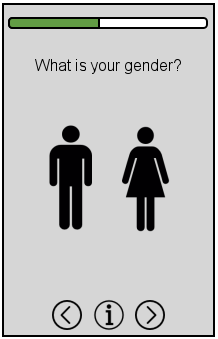
\includegraphics[scale=0.48]{pics/wireframes/plain2-6.png}
      \label{fig:wireframe13}
    }
    \subfigure[Q7: Age]{
      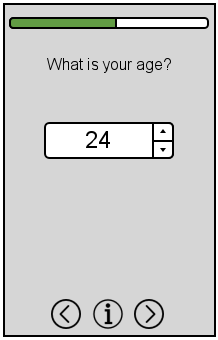
\includegraphics[scale=0.48]{pics/wireframes/plain2-7.png}
      \label{fig:wireframe14}
    }
    \subfigure[Q8: Nationality]{
      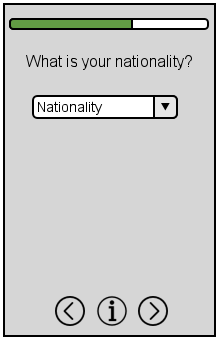
\includegraphics[scale=0.48]{pics/wireframes/plain2-8.png}
      \label{fig:wireframe15}
    }
  \end{figure}

  \begin{figure}
    \centering
    \subfigure[Q9: Android Unlock Pattern experience]{
      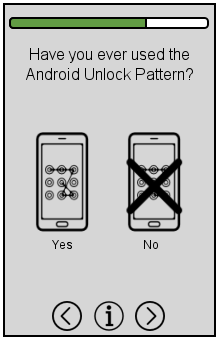
\includegraphics[scale=0.48]{pics/wireframes/plain2-9.png}
      \label{fig:wireframe16}
    }
    \subfigure[Q10: Screen lock usage]{
      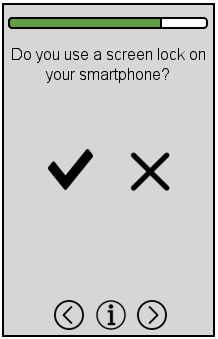
\includegraphics[scale=0.48]{pics/wireframes/plain2-10.png}
      \label{fig:wireframe17}
    }
    \subfigure[Q11: Selected screen lock]{
      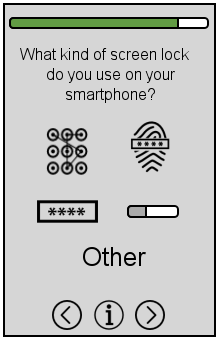
\includegraphics[scale=0.48]{pics/wireframes/plain2-11.png}
      \label{fig:wireframe18}
    }
    \subfigure[Q12: Mobile OS]{
      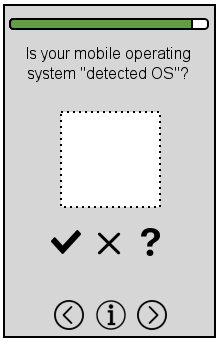
\includegraphics[scale=0.48]{pics/wireframes/plain2-12.png}
      \label{fig:wireframe19}
    }
    \subfigure[Q13: Experience with IT and security]{
      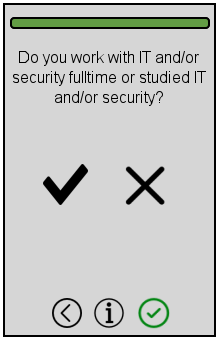
\includegraphics[scale=0.48]{pics/wireframes/plain2-13.png}
      \label{fig:wireframe20}
    }
    \subfigure[Questionnaire completed]{
      
\includegraphics[scale=0.48]{pics/wireframes/plain2-14.png}
      \label{fig:wireframe21}
    }
    \caption{Wireframes}
    \label{fig:wireframes}
  \end{figure}

